\documentclass[a4paper, 11pt]{scrartcl}
\usepackage[utf8]{inputenc}
\usepackage[ngerman]{babel}
\renewcommand{\familydefault}{\sfdefault}
\usepackage[a4paper]{geometry}
\usepackage{hyperref}
\usepackage{graphicx}
\usepackage[usenames,dvipsnames,svgnames]{xcolor}
\usepackage{amsmath}
\usepackage{lipsum}
\usepackage{verbatim}
\usepackage{listings}
\usepackage{soul}
\usepackage{titlesec}
\usepackage{booktabs}
\usepackage{multirow}
\usepackage{graphicx}

% Serifenfont für Überschriften
\setkomafont{disposition}{\normalcolor\bfseries}
% Seitengröße mit Geometry-Paket einstellen
\geometry{left=2.75cm,right=2.75cm,top=23mm,bottom=25mm,head=14.5pt}

\sethlcolor{lightgray}
\newcommand{\inlinecode}[1]{\hl{\texttt{#1}}}
\newcommand{\todo}[1]{\textbf{\color{red}{#1}}\normalcolor}

\title{Datenbankpraktikum -- Gruppe 3\\ Übungsblatt 5 Aufgabe 1}
\author{Janis Hamme, Karoly Kemeny, Thomas Neureuther,\\ Ming Niu, Alex Rubinshteyn,  Xinxin Yang}

\lstset{
    frame=top,frame=bottom,
    breaklines=true,
    captionpos=t,
    inputencoding={utf8},
    columns=fullflexible,
    breaklines=true
}

\lstset{literate=%
{Ö}{{\"O}}1
{Ä}{{\"A}}1
{Ü}{{\"U}}1
{ß}{{\ss}}2
{ü}{{\"u}}1
{ä}{{\"a}}1
{ö}{{\"o}}1
}


\titlelabel{\thetitle. }

\usepackage{parskip}
\setlength{\parindent}{0pt}
\setlength{\parskip}{0.5em}

\begin{document}

\maketitle

\section{Teilaufgabe}

Nachdem die Umgebungsvariablen für Hadoop und Hive eingerichtet wurden kann man mit dem Kommando \inlinecode{beeline -u jdbc:hive2://} auf eine Hive Shell zugreifen.

Bei Hive wird zwischen \emph{managed} und \emph{external} Tabellen unterschieden. Bei managed Tabellen wird der Datenbestand von Hive selbst in einem Warehouse verwaltet während mit externen Tabellen bereits im HDFS existierende Daten eingebunden werden können. Da für das spätere Clustering direkt auf die Daten zugegriffen werden muss, sollte hier eine externe Tabelle verwendet werden.

Das gegebene Text-Datenformat der \emph{Word2Vec}-Datenbestände kann direkt als Datenquelle für eine Hive Tabellen dienen: ein Datensatz belegt jeweils eine Zeile, wobei Wörter von ihrem zugehörigem Vektor durch einen Doppelpunkt, und einzelne Einträge des Vektors durch ein Komma, getrennt sind. \autoref{lst:schema} enthält SQL Code um eine entsprechende Tabelle anzulegen.

\lstinputlisting[language=SQL,breaklines=true,caption=Schema,label=lst:schema]{../../Hive/SQL/schema.sql}

Im Hinblick auf das Clustering wird ein spezielles Feld für Partitions-IDs benötigt welches über den Dateipfad abgebildet wird. Ein Datensatz lässt sich importieren indem er an den korrekten Pfad kopiert wird. Beispielsweise durch den Befehl \inlinecode{hdfs dfs -cp /usr/local/hadoop/dbprak/public/example.txt /usr/local/hadoop/dbprak/group3/words/id=0/example.txt}.

\lstinputlisting[language=SQL,breaklines=true,caption=Query,label=lst:query]{../../Hive/SQL/queries.sql}

\autoref{lst:query} zeigt wie eine typische Anfrage an die Tabelle aussehen könnte um die 50 ähnlichsten Wörter zu finden. Dazu muss allerdings zunächst eine Metrik, in diesem Falle \emph{cosineSimilarity}, als Userdefined Function implementiert werden. Da sowohl der Vektor des angefragten Wortes als auch des jeweils anderen Wortes als Parameter benötigt wird ist ein Cross Join notwendig.
\section{Teilaufgabe}

\subsection{k-Means Map und Reduce Pseudocode}
K-Means ist einer der bekanntesten Algorithmen zur Clusteranalyse. Dabei werden ähnliche Objekte zu einer Gruppe zusammengefasst. Die Ähnlichkeit wird durch den Abstand im Raum (Distanz) repräsentiert. 

Zu Beginn erwartet k-Means die Anzahl \emph{k} der gewünschten Cluster und erstellt daraufhin \emph{k} initiale Clusterzentren auf dem übergebenen Datensatz.

\begin{figure}[htb]
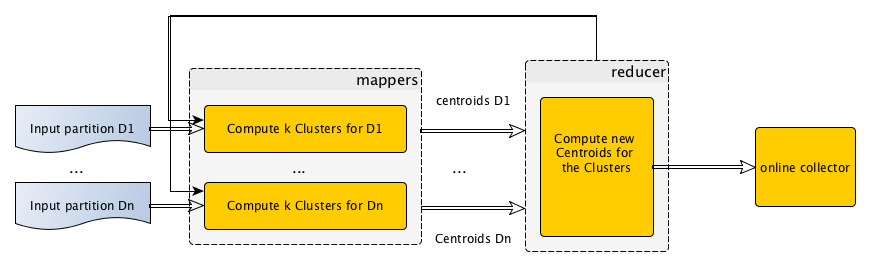
\includegraphics[scale=0.5]{MapReduceBild.png}
\centering
\caption{Überblick über die MapReduce Ausführug von k-Means}
\label{fig:MapRed}
\end{figure}

\subsubsection{Map}
Im Map-Schritt werden die Datenpunkte (WordVektoren) den Clustern zugewiesen. Als Output werden Key-Value-Paare mit dem Cluster als Key erwartet. 
\begin{lstlisting}[caption=Map Pseudocode,label=lst:map,numbers=left,xleftmargin=2em,
framexleftmargin=2em,morekeywords={FOREACH, IF, NULL}]

// Gegeben: Liste mit k initialen Clusterzentren, unsere Word-Vektoren
// Mit der Map-Funktion werden die Clusterzentren und ein Teil der Word-Vektoren als Argumente übergeben

Map (List<ClusterCenter> centers, List<WordVector> words) 

  FOREACH wordVector in words {
  
    minDistance = Double.MaxValue;
    nearestClusterCenter = NULL;  
  
    FOREACH center in centers {
      //Distanzmessung wie in Userdefined Function Cosinus-Ähnlichkeit 
      distance = measureDistance(center, word);
      IF(distance < minDistance) {
        minDistance = distance;
        nearestClusterCenter = center;
      }
    }
    
    //Speichere KeyValue Pair also WordVector zu dem Clusterzentrum 
    context.write(nearestClusterCenter, wordVector);
  }
}
\end{lstlisting}

\subsubsection{Reduce}

Im Reduce-Schritt werden für die Datenpunkte (WordVektoren) die Clustermittelpunkte berechnet und gespeichert. Der Input für den Reducer ist der sortierte Output des Mappers, also die Clusterzuordnungen. .
\begin{lstlisting}[caption=Reduce Pseudocode,label=lst:reduce,numbers=left,xleftmargin=2em,framexleftmargin=2em]
public void reducer(ClusterCenter key, Iterable<WordVector> values, Context context)
{
 //Summiere alle Vektoren auf
 vectorSum = null;
 FOREACH WordVektor in Wordvectors{
   VectorSum += Wordvector; 
 }
 
 CenterVector = VectorSum/VectorCount;
 CenterId = ClusterCenter.id;
 //Speichere KeyValue Pair also CenterId und Vector
 context.write(CenterId, CenterVector)
 //Zähler für Endbedingung
 context.UpdateCount;
 
}
\end{lstlisting}

\subsection{Initialisierung der Algorithmen}
Zu Beginn der Ausführung müssen die Clusterzentren initialisiert werden. Dabei wird für die gewünschte Anzahl an Clustern jeweils ein zufälliger Punkt als Clusterzentrum gewählt. Dafür muss der Seed in der Initialisierung gesetzt werden. Im laufe der Iterationen verscheiben sich diese dann immer stärker zu den eigentlichen Clusterzentren.

\subsection{Klassen und Methoden}
Für die Implementierung von Map-Reduce-Anwendungen werden einige User-Interfaces bereitgestellt. Anwendungen wie z.B. WordCount implementieren typischerweise die \textit{Map-} und \textit{Reduce-Klassen}. Die Map und die Reduce-Klasse werden in der Main-Methode über \textit{Job.setMapper(class)} bzw. \textit{Job.setReducer(class)}  gesetzt. Dies ist auch für den K-Means Algorithmus notwendig.

Für jeden InputSplit im InportFormat wird ein Job gestartet.

Die \textit{Mapper Klasse} soll neben der Map Schritt auch weitere Methoden zu implementieren. In der \textit{Setup-Methode} werden die notwendigen Initialisierungen vorgenommen und die Konfiguration durchgeführt. Auch eine Parse-Methode wird zum analysieren des Inputs benötigt. Für die Berechnung der Distanz im Map-Schritt ist eine Distanzmesser zu implementieren.

Die \textit{Reducer-Klasse} enthält die \textit{Reduce-Methode} welche die Clustermittelpunkte bilden soll.

Außerdem ist es für den Anwendungsfall sinnvoll ein Modell zu implementieren. Dies ist im WordCount-Beispiel nicht zu finden, was der Einfachheit des Beispiels geschuldet ist. Dies wird in der Main-Methode 			\textit{job.setOutputKeyClass(class)} und \textit{job.setOutputValueClass(class)} gesetzt. Sinvolle Klassen wären ClusterCenter und WordVector.

\section{Teilaufgabe}

\subsection{Generelles}

% Wegen Ressourcenbeschränkungen können wir für jeder Anfrage nicht Alle Worte in unserem Wortsatz untersuchen ob sie geeignet für Vorschlag sind. Deshalb möchten wir Clustering einsetzen, um die Suchraum zu beschränken. Am Ende kann man das Ergebnisse als True Positive wahrnehmen, wenn es eine Synonyme, Hyponyme oder Hyperonyme ist, mit diesem ansatz können wir die Genauigkeit von dem Clustering mit einem ROC Kurve aufzeigen.
%
%Für diese Projekt benutzen wir Word2Vec als ausgangspunkt für Clustering, weil wir gehört haben, dass es auch Semantische relationen zwischen Worte erkennen kann. Um den Clustering auszuwerten werden wir Wordnet benutzen (siehe nächste Paragraph).

Die lexikalische Datenbank Wordnet gruppiert die enthaltenen Wörter in Synonymgruppen (\emph{Synsets})  verschiedener Sprachbereiche (Nomen, Adjektiven, Verben und Adverben). Diese werden auf verschiedene Art und Weise in Relation gesetzt. Mit Hilfe von Wordnet soll untersucht werden ob die durch Word2Vec gebildeten semantischen Beziehungen für einen Recommender geeignet sind.

Für die Resultate eines Recommenders sind hauptsächlich Synonyme, Hyponyme und Hyperonyme nützlich, da den Kunden so ähnliche Produkte vorschlagen werden sollen. Da aufgrund beschränkter Ressourcen, Anfragen auf einen Cluster beschränkt werden sollen, muss untersucht werden wie stark die Ergebnisqualität dadurch beeinflusst wird.

\subsection{Zu untersuchende Zusammenhänge}

%\todo{Notizen von hier und von Karoly fertig ausformulieren}

\subsubsection{Enthaltene Relationen sind (je nach Wortart)}

\begin{itemize}
\item{Hierarchische Anordnung von Synsets in Mengen von Überbegriffen (Hyperonyme) und Unterbegriffen (Hyponyme)}
\item{Teil-Ganzes Beziehungen zwischen Synsets}
\item{Spezialisierungen von Verben}
\item{Gegenteile für Adjektive}
\end{itemize}

\subsubsection{Beispiele zur Motivation}

\begin{itemize}
\item{Gesucht: soft sweater}
\item{Gute Vorschläge: comfortable sweater, soft pullover, fleecy hoodie}
\item{Schlechte Vorschläge: scratchy sweater}
\end{itemize}

\subsubsection{Dabei zu berücksichtigen}

\begin{itemize}
\item{Welche Suchbegriffe eignen sich für die Untersuchung? $\rightarrow$ Testbegriffe festlegen}
\item{Wie viele ähnliche Begriffe finden sich überhaupt in der Wordnet Datenbank (Überdeckung) $\rightarrow$ (Begriffe filtern?)}
\item{Semantische Zusammenhänge: Synonyme, Hyponyme und Hyperonyme allgemein als erwünschter Bestandteil (bei jeder Wortart), bei Adjektiven aber keine Antonyme $\rightarrow$ Statistiken erstellen um Qualität der Ergebnisse zu prüfen}
\item{Auswirkungen des Clusterings auf die Ergebnisqualität evaluieren und optimale Clustergröße ermitteln (Qualität/Performance Trade-off)}
\end{itemize}

\subsection{Umsetzung in Java}

%\todo{Notizen von hier und von Karoly fertig ausformulieren}

%\begin{itemize}
%\item{nicht auf spezifische Wordnet Library festlegen, aber darauf hinweisen, dass verschiedene existieren}
%\item{Verbindung zu Hive über JDBC}
%\item{Nutzung eines vordefinierten Testsets an Wörtern}
%\item{Ergebnisse in textueller Form}
%\end{itemize}

\begin{itemize}
\item{Java Bibliotheken für Wordnet nutzen (z.B. JAWS $\rightarrow$ Java API for WordNet searching.)}
\item{Testwörter aus Datei einlesen und Anfragen für jedes Wort mit und ohne Clustering ausführen}
\item{Verbindung zu Hive aus Java über JDBC.}
\item{Ausgabe des Ergebnises in Textform.}
\end{itemize}
\newpage
\section*{Zeitplanung und Rollenverteilung}

\begin{center}
\begin{tabular}{llr}
\multicolumn{3}{c}{\hfill} \\
\multicolumn{3}{l}{\makebox[\textwidth][l]{\textbf{Beginn Implementierungsphase}}} \\
\toprule
\emph{15.12.2015} & \multicolumn{2}{l}{\textbf{Java Projekte einrichten}} \\
& Hive Userdefined Function & Alex und Janis \\
& Map-Reduce Clustering & Thomas und Karoly \\
& Evaluation mit Wordnet & Ming und Xinxin \\
\cmidrule{1-3}
\emph{24.12.2015} & \textbf{*Weihnachtsferien*} & \multirow{3}{*}{Verteilung wie oben} \\
& Mit Java Libraries vertraut machen & \\
& Prototyping & \\
\cmidrule{1-3}
\emph{07.1.2016} & \textbf{Team Meeting} & \multirow{3}{*}{Alle} \\
& Ergebnisse anderen Team-Mitgliedern präsentieren\hspace{-3em} & \\
& Offene Probleme besprechen und lösen & \\
\cmidrule{2-3}
& \textbf{Beginn Implementierung Teil 1} & \\
& Hive Userdefined Function & Alex, Janis und Ming  \\
& Map-Reduce Clustering & Thomas, Karoly und Xinxin \\
\cmidrule{1-3}
\emph{12.01.2016} & \textbf{Team Meeting} & \\
%\cmidrule{2-3}
& \textbf{Abschluss Implementierung Teil 1} & \\
\cmidrule{2-3}
& \textbf{Beginn Implementierung Teil 2} & \multirow{3}{*}{Alle} \\
& Evaluation mit Wordnet & \\
& Optimierung und Fehlerkorrektur von Teil 1& \\
\cmidrule{1-3}
\emph{17.01.2015} & \textbf{Team Meeting} & \\
& \textbf{Abschluss Implementierung Teil 2} & \multirow{3}{*}{Alle} \\
& Letze Verbesserungen & \\
& Zeitpuffer &  \\
\cmidrule{1-3}
\emph{26.-29.1.2015} & \textbf{Code-Review} & Alle \\
\bottomrule
\end{tabular}
\end{center}


\begin{center}
\begin{tabular}{llr}
\multicolumn{3}{c}{\hfill} \\
\multicolumn{3}{l}{\makebox[\textwidth][l]{\textbf{Beginn Evaluationsphase}}} \\
\toprule
\emph{26.2.2016} & \textbf{Team Meeting} & \multirow{3}{*}{Alle} \\
& Vorschläge für Anfragen sammeln (3 Stück festlegen) & \\
& Methodik zur Performance Messung festlegen & \\
\cmidrule{2-3}
& \textbf{Beginn Messungen und Aufbereitung der Ergebnisse (Handout)} & 2er-Teams\\
\cmidrule{1-3}
\emph{02.2.2016} & \textbf{Team Meeting} & \multirow{2}{*}{Alle} \\
& Ergebnisse vorstellen & \\
\cmidrule{2-3}
& \textbf{Präsentation erstellen} & 2er-Teams \\
\cmidrule{1-3}
\emph{09.2.2016} & Abschlusspräsentation & Alle \\
\bottomrule
\end{tabular}
\end{center}

\end{document}
